\documentclass[9pt]{beamer}
%\documentclass[handout]{beamer}

\mode<presentation>
{
  \usetheme{default}      % or try Darmstadt, Madrid, Warsaw, ...
  \usecolortheme{default} % or try albatross, beaver, crane, ...
  \usefonttheme{serif}  % or try serif, structurebold, ...
  \setbeamertemplate{navigation symbols}{}
  \setbeamertemplate{caption}[numbered]
  \usefonttheme{structuresmallcapsserif}
}

\newcommand{\Prob}{\text{Prob}}
\newcommand{\bx}{\mathbf{x}}
\newcommand{\bphi}{\pmb{\phi}}
\newcommand{\btheta}{\pmb{\theta}}
\newcommand{\Count}{\text{count}}
\newcommand{\given}{\, | \,}
\newcommand{\diag}{\text{diag}}
\DeclareMathOperator*{\argmax}{arg\,max}

%\usepackage{pgfpages}
%\pgfpagesuselayout{4 on 1}[a4paper,border shrink=5mm]

\title{A Brief on Natural Language Processing}
\author{Luis Berlioz}
\begin{document}
\maketitle


%%%%FRAME
\begin{frame}{arXiV Website bulk download}
    \begin{columns}[T]
        \begin{column}{0.4\textwidth}
    
\includegraphics[width=\textwidth]{bulk_download.png} 
        \end{column}
        \begin{column}{0.6\textwidth}
            \begin{itemize}
                \item About 885 Gigabytes of .tar files.
                \item Each .tar file is about 500 Megabytes.
                \item \texttt{tar -tvf arXiv\_src\_1806\_033.tar}
                    \begin{itemize}
\item \hspace{4em}      $\vdots$
\item 1806/1806.11561.gz
\item 1806/1806.11543.gz
\item 1806/1806.11557.pdf
\item 1806/1806.11567.gz
\item 1806/1806.11568.gz
\item \hspace{4em}      $\vdots$
\end{itemize}


            \end{itemize}
        \end{column}
    \end{columns}
\end{frame}


%%%%FRAME
\begin{frame}{Metadata API}
    ArXiv gives access to all the data they display on the website:
    \begin{columns}[T]
        \begin{column}{0.4\textwidth}
    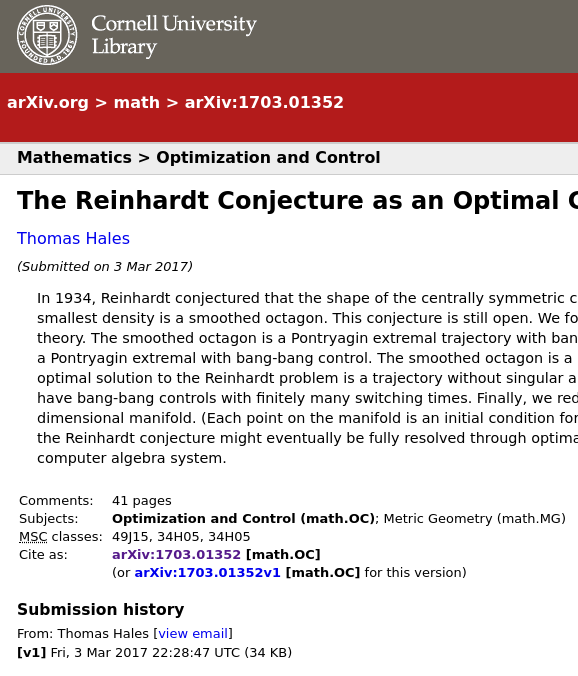
\includegraphics[width=\textwidth]{hales_article.png} 
        \end{column}
        \begin{column}{0.6\textwidth}
            \begin{itemize}
                \item \textbf{id:} http://arxiv.org/abs/1703.01352v1
                \item \textbf{published:} 2017-03-03T22:28:47Z
                \item \textbf{updated:} 2017-03-03T22:28:47Z
                \item \textbf{title:} ``The Reinhardt Conjecture as an Optimal Control Problem''
                \item \textbf{summary:} ``In 1934, Reinhardt conjectured that the shape of \ldots''
                \item \textbf{authors:} ['Thomas Hales', ] 
                \item \textbf{arxiv\_primary\_category:} math.OC (Optimal Control)
                \item \textbf{49J15:} Optimal control problems involving ordinary differential equations
                        \item ``Secondary category'': math.MG (Metric Geometry)
                        \item \textbf{34H05:} Ordinary differential equations, Control problems.
                    \end{itemize}
        \end{column}
    \end{columns}
\end{frame}

%%%%FRAME
\begin{frame}{Some arXiV.org website stats}
    \begin{columns}[T]
        \begin{column}{0.5\textwidth}
    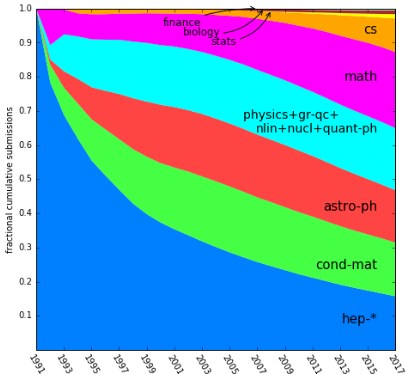
\includegraphics[width=\textwidth]{cum_submissions.png} 
        \end{column}
        \begin{column}{0.5\textwidth}
		\resizebox{\columnwidth}{!} & \textbf{Curr. \%} \\
		\hline
		\color{purple}{math+math-ph} & 299,046 & 22.3\% & 25.6\% \\
		\hline
		\color{blue}{hep} & 212,905 & 15.9\% & 7.8\% \\
		\hline
            \color{green}{cond-mat} & 210,802 & 15.7\% & 11.7\% \\
		\hline
            \color{red}{astro-ph} & 205,424 & 15.3\% & 10.7\% \\
		\hline
		\color{orange}{cs} & 132,409 & 9.9\% & 21.9\% \\
		\hline
		physics & 88,632 & 6.6\% & 8.6\% \\
		\hline
			\end{tabular}}
            \begin{figure}[h]
    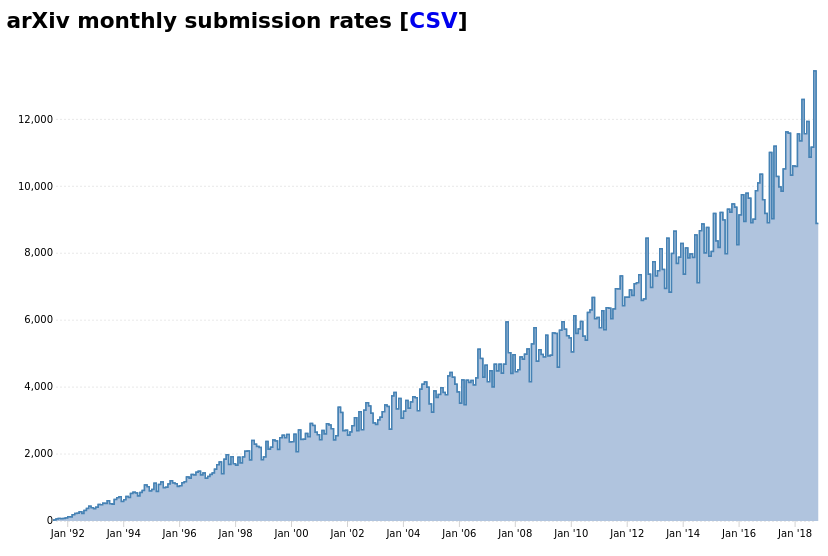
\includegraphics[width=\textwidth]{subm_rates.png} 
            \end{figure}
			\end{column}
			\end{columns}
\end{frame}

%%%%FRAME
\begin{frame}{LaTeXML Website and github stats}
    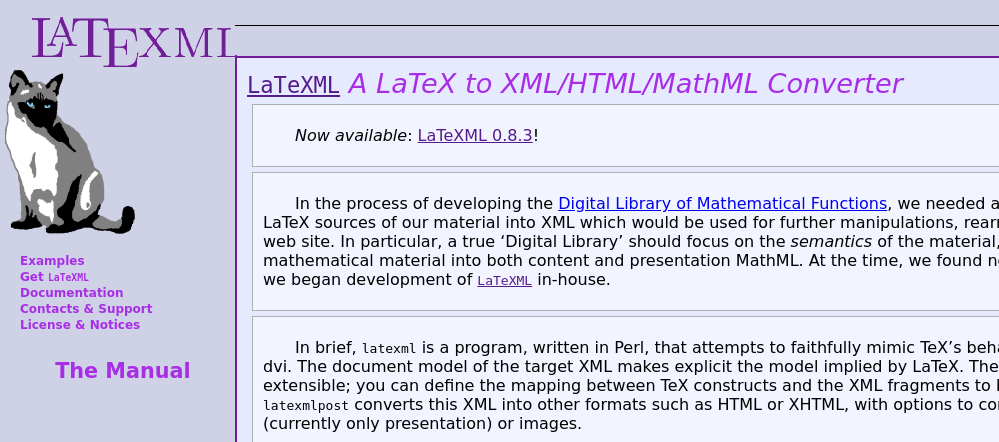
\includegraphics[width=0.9\textwidth]{ltxml_website.png}
    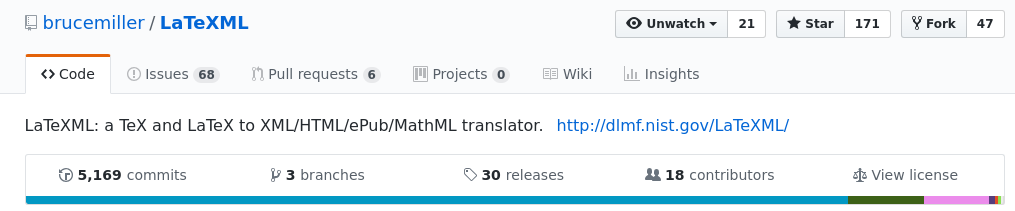
\includegraphics[width=0.9\textwidth]{ltxml_github1.png}
    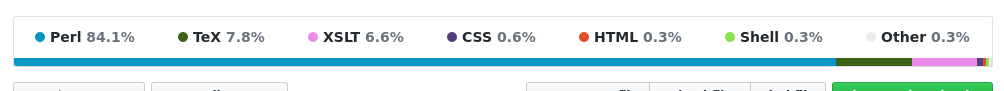
\includegraphics[width=0.9\textwidth]{ltxml_github2.png}
\end{frame}

%%%%FRAME
\begin{frame}{LaTeXML Short Demo}
    \begin{columns}[T]
        \begin{column}{0.5\textwidth}
    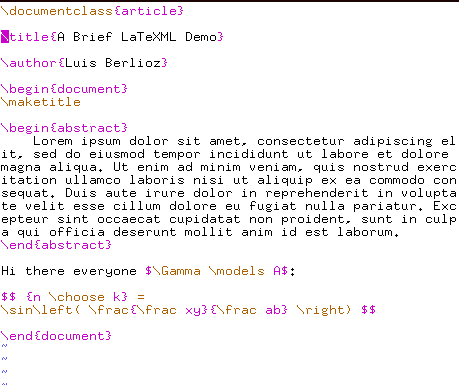
\includegraphics[width=\textwidth]{ltxml_demo_vim.png}
    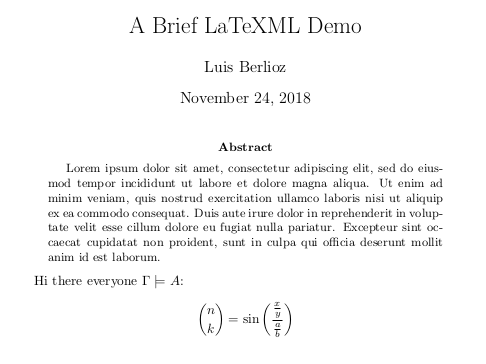
\includegraphics[width=\textwidth]{demo_pdf.png}
        \end{column}
        \begin{column}{0.5\textwidth}
    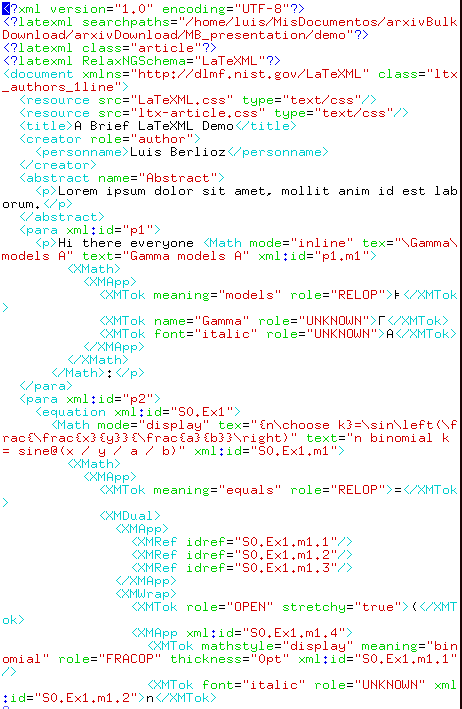
\includegraphics[width=\textwidth]{ltx_demo_output.png}
        \end{column}
    \end{columns}
\end{frame}

%%%%FRAME
\begin{frame}{Natural Language Processing (NLP)}
    Using Machine Learning techniques with Human Language.
    \begin{itemize}
            \item AKA Computational Linguistics.
            \item Goes from a continuous medium (airwaves) to a discrete (text).
        \item Traditionally, speech processing is done by electrical engineers and NLP by C.S. people.
            \item Really complex, consider the following headline:
                \begin{itemize}
                    \item \textit{``Scientists study whales from space.''}
                \end{itemize}
    \item No A.I. program could be said to be complete without the ability to communicate in words.
        \item Important role in Search and Text Mining.
    \end{itemize}
     
\end{frame}


%%%%FRAME
\begin{frame}{Dependency Parsing}
    \begin{itemize}
            \item Binary Asymmetric relations between words.
            \item Typed with the name of the grammatical relation.
            \item Arrow points to the dependent.
            \item Usually forms a connected, acyclic tree with a unique head.
    \end{itemize}
\end{frame}

 %%%%FRAME
\begin{frame}{Common Terminology for Classification Problemks}
    \begin{exampleblock}{Vocabulary}
        The set $V = \{w_1,w_2,\ldots, w_V\}$ of all the \textit{words} or \textit{tokens}.
    \end{exampleblock}
        \begin{itemize}
            \item \textbf{Common Crawl (uncased)} 42B tokens, 1.9M vocab.
            \item \textbf{Common Crawl (cased)} 840B tokens, 2.2M vocab.
            \item \textbf{Twitter} 2B tweets, 27B tokens, 1.2M vocab
            \item \textbf{Wikipedia 2014 + Gigaword 5} 6B tokens 400K vocab
            \item \textbf{arXiv.org} 1,000,295 vocab.arxmliv.txt
        \end{itemize}

        \begin{exampleblock}{Labels or Classes}
            The set of labels $\{y^{(1)},y^{(2)},\ldots, y^{(n)}\}$\\
            In the example these were: \textbf{Definitions, Examples, Propositions, etc}.
        \end{exampleblock}


\end{frame}

\begin{frame}{Bag of Words Model}
    Represent a document, email, tweet as a vector $\bx=(x_1,\ldots, x_V)$
    \begin{columns}[T]
        \begin{column}{0.6\textwidth}
            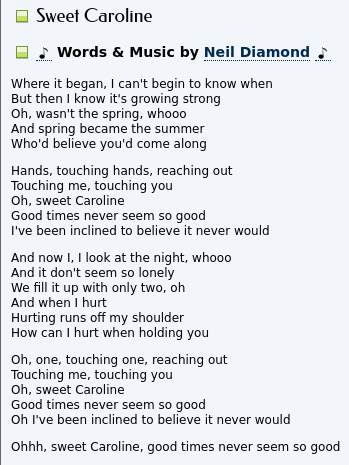
\includegraphics[width=0.9\textwidth]{sweet_caroline_lyrics.png}
        \end{column}
        \begin{column}{0.4\textwidth}
            \begin{tabular}{|c|l|c|}
                \hline
                \hline
                $V$ & TOK& Freq. \\
                \hline
                \hline
                23 & oh&6\\
                \hline
                4500 & touching&6\\
                \hline
                10 & good&6\\
                \hline
                80 & never&5\\
                \hline
                50 & seem&4\\
                \hline
                38 & believe&3\\
                \hline
                99 & sweet&3\\
                \hline
                43 & caroline&3\\
                \hline
                30 & time&3\\
                \hline
                90 &know&2\\
                \hline
                54& spring&2\\
                \hline
                897& whooo&2\\
                \hline
                230 & hand&2\\
                \hline
                654 & reaching&2\\
                \hline
            \end{tabular}
        \end{column}
    \end{columns}
\end{frame}


\begin{frame}{Similarity based representations}
    \begin{block}{One-hot Representation}
        It has 1 in index of the word and 0 elsewhere
        $$\text{word} \mapsto [0,0,0,\ldots,0,1,0,\ldots,0,0,0,0]$$
        But we would like:
        \begin{itemize}
            \item Lower dimension.
            \item Similar words are close by.
        \end{itemize}
    \end{block}



\end{frame}

%%%%FRAME
\begin{frame}{Co-ocurrence Matrix}
    \textit{``You shall know a word by the company it keeps''}\\[4mm]
    \hspace*\fill{\small John R. Firth}
    \begin{figure}[c]
    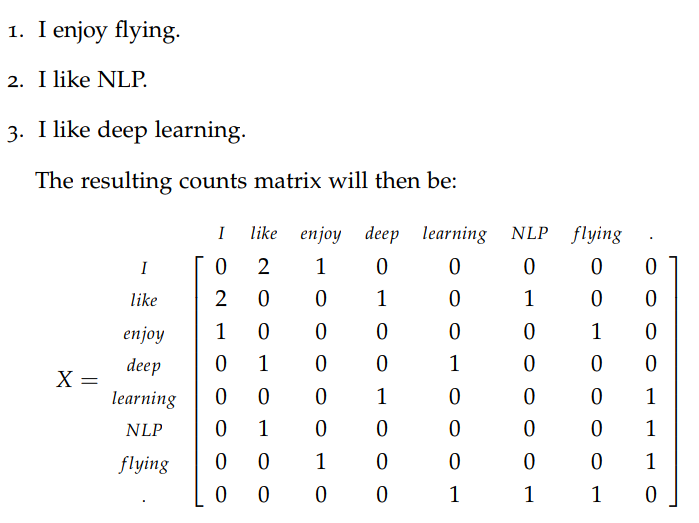
\includegraphics[width=0.75\textwidth]{coocurrence_matrix.png}
    \end{figure}
    \begin{itemize}
        \item Observe that \textit{like} and \textit{enjoy} are NOT orthogonal.
    \end{itemize}
\end{frame}

%%%%FRAME
\begin{frame}{Co-ocurrence Matrix}
Let $X = U\Sigma W^T$ be the SVD of $X$
    $$ U = [u_1 \given u_2\given \cdots ]\quad \Sigma = \diag(\sigma_1,\ldots, \sigma_V)\quad W = \begin{bmatrix}-& w_1&- \\-& w_2&- \\ &\vdots& \end{bmatrix}$$
        Approximate $X$ by taking $k<V$ singular values:
        $$\hat X = \sum_{t=1}^k \sigma_t\, u_k\, W_k^T\approx X$$
        \begin{itemize}
                \item Above, $W_k^T$ are the columns of $W$.
        \item The one-hot vector are embedded in $k$-dimensional space as the vectors $\bar w_k^T$.
        \end{itemize}
\end{frame}

\begin{frame}{Similarity based representations}
    If $w_t$ is the word we care about and $w_{t +j}$ denotes the words to the left or right:
    $$\Prob(w_{t+j}\given w_t)$$
    \begin{itemize}
        \item $\Prob(w_{t-1}=\text{cauchy} \given w_t=\text{sequence})$ should be high.
        \item $\Prob(w_{t+1}=\text{infinite} \given w_t=\text{finite})$ should be very low.
    \end{itemize}
    \begin{figure}[c]
    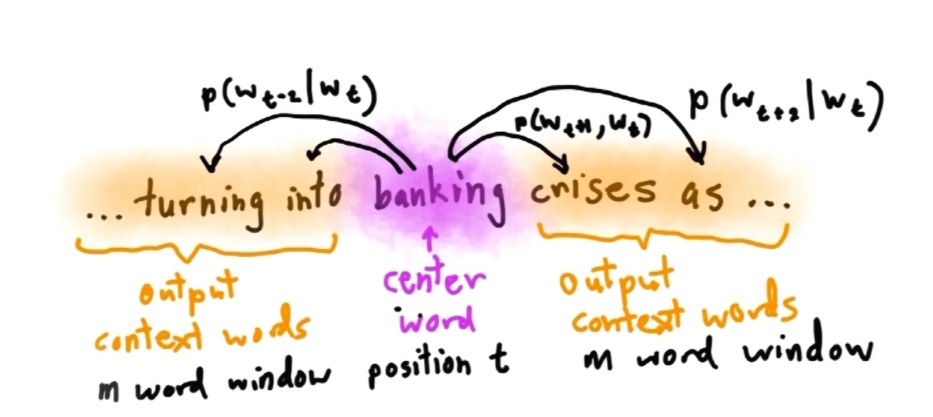
\includegraphics[width=0.7\textwidth]{skipgram.png}
    \end{figure}
\end{frame}

%%%%FRAME
\begin{frame}{Setup of Skip-Gram}
    Given a word $w_t$ we want to predict its \textit{context:} $$C_{w_t} = \{w_{t+j} :\ |j|\leq m \text{ and } j \neq 0\}$$
    $$\hat J(\btheta) = \prod_{t=1}^T\  \prod_{\substack{|j|\leq m\\ j\neq 0}} \Prob(w_{t+j}\given w_t; \btheta)$$
    $$J(\btheta) = \frac 1T \sum_{t=1}^T \sum_{\substack{|j|\leq m\\ j\neq 0}}\log \Prob(w_{t+j}\given w_t; \btheta)$$
    We want to find $\hat \btheta  = \argmax_{\btheta} J(\btheta)$.
\end{frame}

%%%%FRAME
\begin{frame}{Skip-Gram }
    We use two type of Parameters:
    \begin{itemize}
            \item $v_t$ for estimating $w_t$ as a center word.
            \item $u_{t-m}, \ldots u_{t-1}, u_{t+1}, \ldots , u_{t+m}$ for $w_t$ as a context word.
            \item $\btheta = (U,W)$ are matrices, $v_t = W\, x$ ($x$ is the one-hot representation of $w_t$.)
    \end{itemize}
    $$\prod_{\substack{|j|\leq m\\ j\neq 0}}\Prob(w_{t+j}\given w_t; \btheta) =    \prod_{\substack{|j|\leq m\\ j\neq 0} } \Prob(u_{t+j} \given v_t)$$
    We estimate this last probability as a softmax:
    $$\Prob(u_{t+j}\given v_t) = \frac{\exp(u^T_{t+j}v_t)}{ \sum_{n=1}^V \exp(u_n^T v_n)}$$
\end{frame}

%%%%FRAME
\begin{frame} 
    Remember:
    $$J(\btheta) = \frac 1T \sum_{t=1}^T \sum_{\substack{|j|\leq m\\ j\neq 0}}\log \Prob(w_{t+j}\given w_t; \btheta)$$
    And:
    $$\Prob(u_{t+j}\given v_t) = \frac{\exp(u^T_{t+j}v_t)}{ \sum_{n=1}^V \exp(u_n^T v_n)}$$
     Putting everything together:
     $$ J(U,W) = \sum_{\substack{|j|\leq m\\ j\neq 0}} u_{t+j}^Tv_t - 2m\log \sum_{n=1}^V \exp(u_n^T v_n)$$
\end{frame}


%%%%FRAME
\begin{frame}{GloVe Project}
    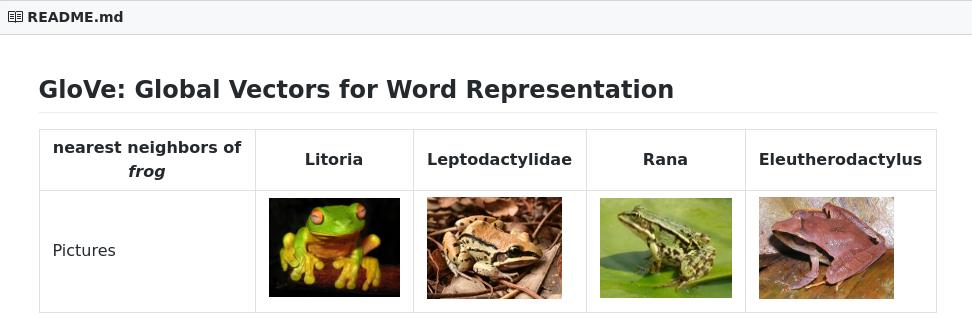
\includegraphics[width=\textwidth]{Glove_github_small.png}

\begin{figure}
   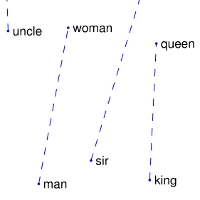
\includegraphics[width=0.29\textwidth]{man_woman_small.jpg}
   \hfill
   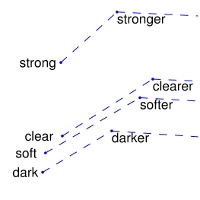
\includegraphics[width=0.29\textwidth]{comparative_superlative_small.jpg}
   \hfill
   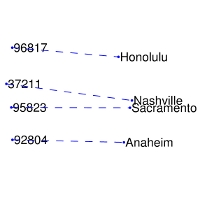
\includegraphics[width=0.29\textwidth]{city_zip_small.jpg}
\end{figure}

\end{frame}
%%%%FRAME
\begin{frame}{Common words and Huge datasets}
    Coping with word frequency and 
    \begin{block}{Sampling Rate}
        Let $w$ be a word and $z(w)$ the ratio at which it appears in the corpus. The probability of keeping the word is:
        $$P(w) = \left(\sqrt{\frac{z(w)}{0.001}} + 1\right) \frac{0.001}{z(w)}$$
For example, $P(w)=1$ when $z(w)\leq 0.0026$.
    \end{block}
    \begin{block}{Negative Sampling}
        The process of selecting a few words that \textbf{do not} show up in the context and updating their weights.
        $$P(w) = \frac{f(w)^{3/4}}{\sum_{j=0}^n f(w_j)^{3/4}}$$
    \end{block}
\end{frame}

%%%%FRAME
\begin{frame}{The Objective functions after Sampling}
    \begin{description}
        \item[Word2Vec:] $\displaystyle J_t(\theta) = \log \sigma(u_o^T v_c) + \sum_{j\sim P(w)}\log \sigma(-u^T_j v_c)$.
        \item[GloVe:] $\displaystyle J(\theta) = \frac 12\sum_{i,j=1}^V f(X_{i\, j}) (u_i^T v_j - \log X_{i\, j})^2$
    \end{description}
    \begin{figure}[b]
    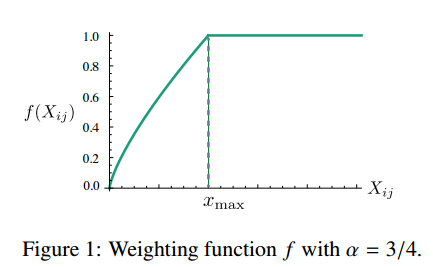
\includegraphics[width=0.6\textwidth]{glove-fig-1.png}
    \end{figure}
\end{frame}
%%%%FRAME
\begin{frame}{Advantages of Similarity based Representation}

    \begin{itemize}
        \item Better classification because similar concepts cluster together.
        \item Sentiment Analysis can actually worsen with word embeddings.
        \item Smaller dimension work better for input to NN.
    \end{itemize}
\end{frame}
\end{document}

